\section{Experiments}
\label{s:experiments}

\vspace{3em}
\begin{table}
\begin{tabular}{cccccc}
Time of Day & Crime & Location & Arrest & Domestic & District \\
\hline
EVENING & BATTERY & RESIDENCE & false & false & 006 \\
NIGHT & NARCOTICS & STREET & true & false & 011\\
NIGHT & THEFT & STREET & false & false & 004\\
EARLY MORNING & CRIMINAL DAMAGE & APARTMENT & false & false & 007\\
EVENING & NARCOTICS & SIDEWALK & true & false & 011\\
NIGHT & BATTERY & APARTMENT & false & true & 006\\
AFTERNOON & THEFT & STREET & false & false & 025\\
MORNING & BURGLARY & RESIDENCE & false & false & 009\\
NIGHT & BATTERY & SIDEWALK & false & false & 012\\
EVENING & BATTERY & RESIDENCE & false & true & 004\\
\hline
\end{tabular}
\caption{Example representatives}
\label{tab:exreps}
\end{table}
\vspace{3em}

Semantically, we found that our system's results were reasonable. The crimes were well-distributed, repeated crimes were generally quite different (a common feature was that battery would be repeated, with domestic events in the home showing up separately from nondomestic outdoor battery leading to arrest), but also showed that some times of day and districts were more or less likely to contain crime (e.g. few afternoon crimes, multiple representatives from ``bad neighborhoods"). A sample set of 10 representatives is shown, in no particular order, in table \ref{tab:exreps}.

Quantitatively, we tested the performance of our algorithm for several thresholds, finding 10 representatives initialized on 300 entries from the Chicago crime dataset with 2 local processes, as 200 insertions were performed. On each insertion, the central solution corresponding to each threshold was scored, as was the oracle solution found by optimizing over the data found in all local and central files. The raw scores are shown in figure \ref{fig:scores} for each insertion and threshold.

\begin{figure}
    \centering
    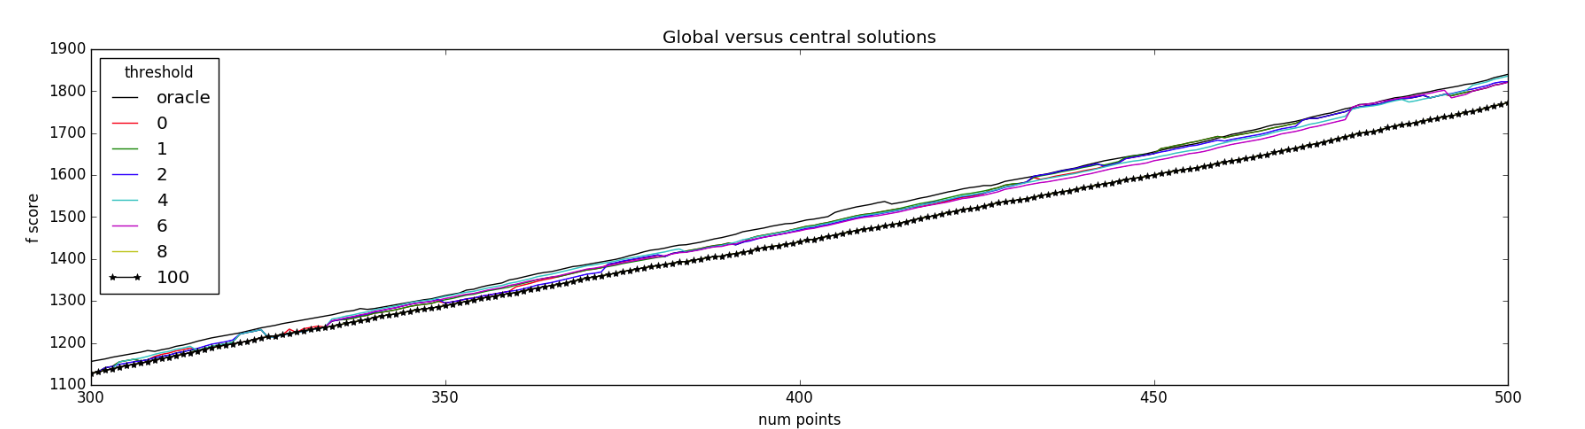
\includegraphics[width=\linewidth]{scores}
    \caption{Raw scores for solutions found under varying thresholds (colors), effectively infinite solution (black with stars), and with access to all data (black line).}
    \label{fig:scores}
\end{figure}

In black, the oracle's solution improves steadily, while in black stars a naive never-update algorithm is shown to perform better than one might expect, given the near-doubling of the dataset. The colored lines in between show that by using a threshold, performance can be increased even to level of the global greedy solution with far less frequent communication. More revealing is the approximation ratio between the oracle and central scores, shown in figure \ref{fig:ratio}.

\begin{figure}
    \centering
    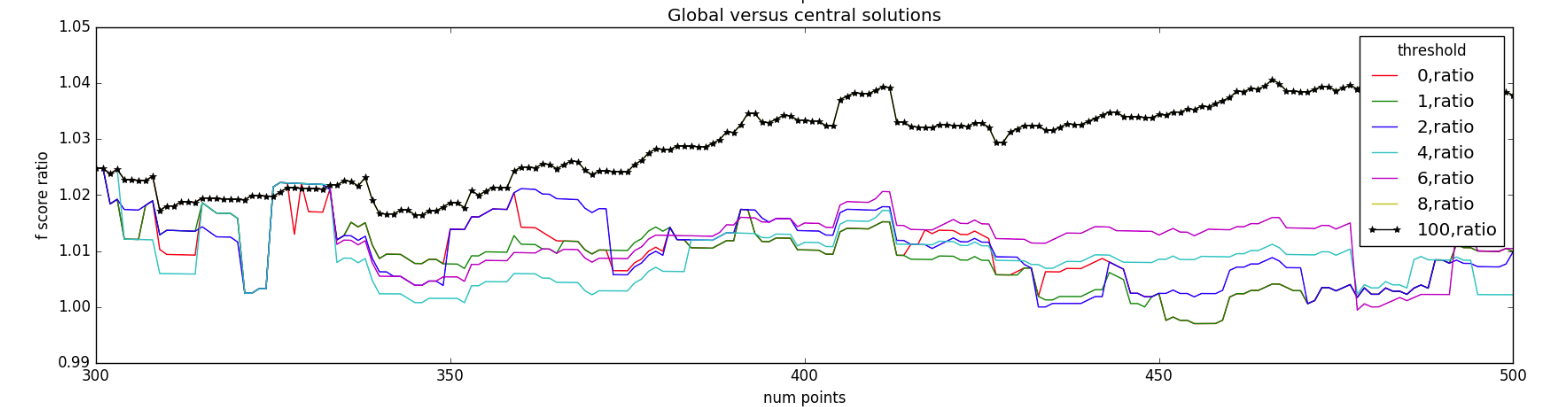
\includegraphics[width=\linewidth]{ratio}
    \caption{Scores from figure \ref{fig:scores}, normalized by oracle score.}
    \label{fig:ratio}
\end{figure}

This measurement, for which 1 is optimal and lower numbers indicate better performance, shows that thresholds improve performance over the naive baseline, though their ordering is fairly variable. We even see the thresholded performance underperforming the naive solution near 330 entries. This plot tells us that a threshold can be expected to usually but not strictly improve performance, and that in the case of this dataset the threshold can exceed half of the representatives (6 changes out of 10) without a serious loss in performance. The threshold of 8 cannot be seen in this plot because it is identical to the naive never-update performance, indicating a major change in behavior between these settings. Finding this tradeoff point for other datasets will determine the lowest communication cost for sensitivity to data changes.